\section{Objectives}
\label{subsec:objectives_formal_modeling_activity}%

The formal modeling activity is carried out using Alloy 6 and aims to validate and ensure the soundness of some of the system’s core processes, with the following aspects as its primary objectives:

\begin{enumerate}

\item \textbf{Consistent System Evolution} \\
We have modeled the rules that define the system's dynamic evolution through time; then, we have defined the intended properties (preconditions and postconditions) of the set of actions, by enforcing role-specific constraints that differentiate their effects depending on who performs them; finally, we have verified that the evolving scenarios remain sound and correct. In particular, in our model we have focused on the following subset of all the possible actions:
\begin{itemize}
 \item Sign Up of a generic User (which can be any of the expected actors: Student, Company or University)
 \item Post a new Internship Offer by a Company
 \item Generate a Recommendation
 \item Accept a Recommendation
 \item Reject a Recommendation
 \item Apply to an Internship Offer
\end{itemize}

\item \textbf{Recommendation Handling Logic} \\
We have defined when Recommendations are generated and how they are linked to Offers and Parties; then, we have modeled the long-lasting effects of actions involving Recommendations; finally, we have ensured state transitions of Recommendations are consistent and irreversible. In particular, every Recommendation generated by the system evolves from an initial \textit{Unhandled} state, eventually becoming either \textit{Accepted} or \textit{Rejected} permanently. 
\end{enumerate}

These are the parts of the system that are, in our opinion, the most critical, as the most complex interactions happen between these functionalities. Given that they have already weighed down the model a lot in terms of the high number of variables and clauses generated during validation, we have decided to avoid modeling other less relevant aspects of the systems (e.g, interview handling), or the possibility of instances being deleted over time, as it would overcomplicate the model while we were trying to achieve a simple and easily understandable representation.

\section{The Model}
\label{subsec:The Model}%

The Model has been structured modularly by separating signatures, actions, facts and the actual worlds in different files.

\subsection{Signatures}

This file contains the definitions of the Signatures of the main entities: a hierarchy of Users (Universities and Parties, with the latter further splitting into Students and Companies), and then Offers and Recommendations. Their fields have been placed by prioritizing \textit{one} as the cardinality of the relation whenever possible, in order to avoid performance overhead and complexity caused by avoidable quantifiers. As an example, \textit{var offeringCompany: one Company} in \textit{sig Offer} has been preferred instead of defining a \textit{var offers: set Offer} field inside \textit{sig Company}.
For every Signature, rules are specified as constraints to ensure that all the instances are always meaningful and consistent: further details about each constraint are commented out in the code.

\lstinputlisting[language=alloy]{Alloy/signatures.als}

\subsection{Actions}

This file contains the modeling of the chosen actions, which have been defined as predicates that, in every time instant, are true if executed and false otherwise. For each action, preconditions that need to hold for it to be executed are conjoined with its postconditions, which are the effects of that specific action to be visible in the next state of the system. Some actions, as has been explained previously in the Use Cases, "call" other ones during their execution: this is the case, for example, for a Student accepting a Recommendation (which means that the system shall automatically make them apply to the corresponding Offer), or for the generation of Recommendations (which must be done by the system as a consequence of other actions happening).

\lstinputlisting[language=alloy]{Alloy/actions.als}

\subsection{Facts} 

This file contains facts for enforcing the consistency of the world, which mostly ensure that the system evolution only happens throughout the action defined in the previous file, and not spontaneously. Signature-specific constraints are not specified here, as they have already been defined in the \textit{Signatures.als} file.

\lstinputlisting[language=alloy]{Alloy/facts.als}

\subsection{Main}

This file contains two worlds: a smaller, somewhat "predetermined" dynamic world, accurately devised to show all the actions and their effects, and a larger static world, casually generated to show that the system is consistent also for a large number of instances. It also contains a predicate modeling the system's standard behavior, which is not really useful as the analyzer tends to always execute the \textit{doNothing} predicate.

\lstinputlisting[language=alloy]{Alloy/main.als}

\section{Validation through the Model}
\label{subsec:Validation through the Model}%

This section shows a possible instance for each of both static and dynamic scenarios according to the defined signatures, actions and facts, obtained by running the predicated in the \textit{main.als} file. 

\subsection{Instance of the Large Static World}

\begin{figure}[H]
    \begin{center}
        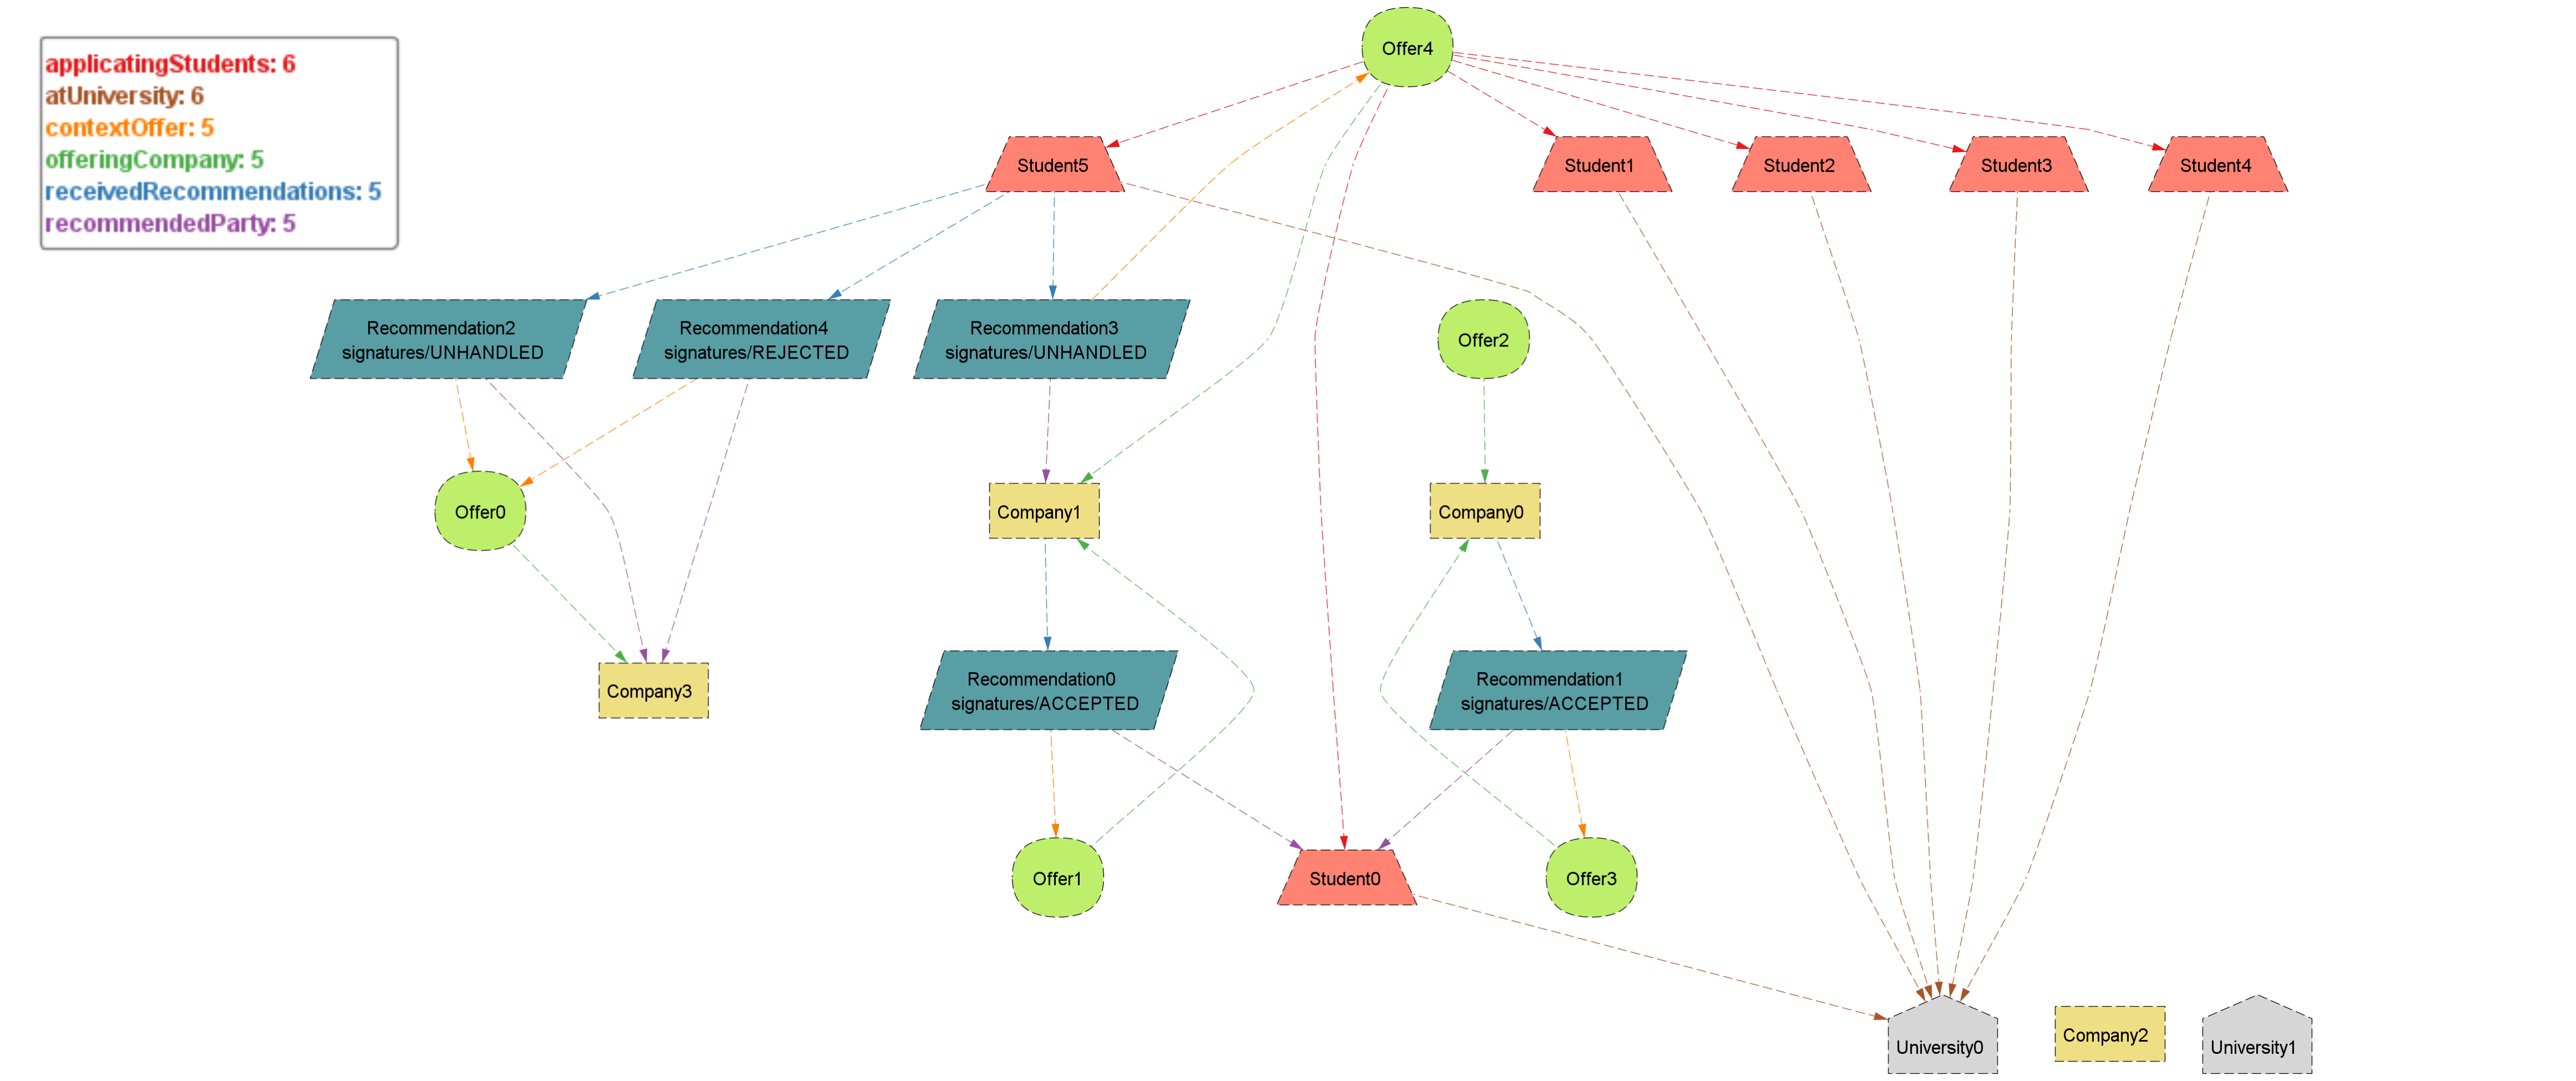
\includegraphics[width=1\linewidth]{LaTeXCode/images/Alloy/largeStaticWorld_high_resolution.png}
        \caption{Large Static World - a meaningful static world spontaneously generated from the Alloy Analyzer, containing a lot of instances and relationships that abide by the static constraints defined.} 
        \label{fig: large_static_world}%
    \end{center}
\end{figure}

\subsection{Instance of the Example Dynamic World}

\begin{figure}[H]
    \begin{center}
        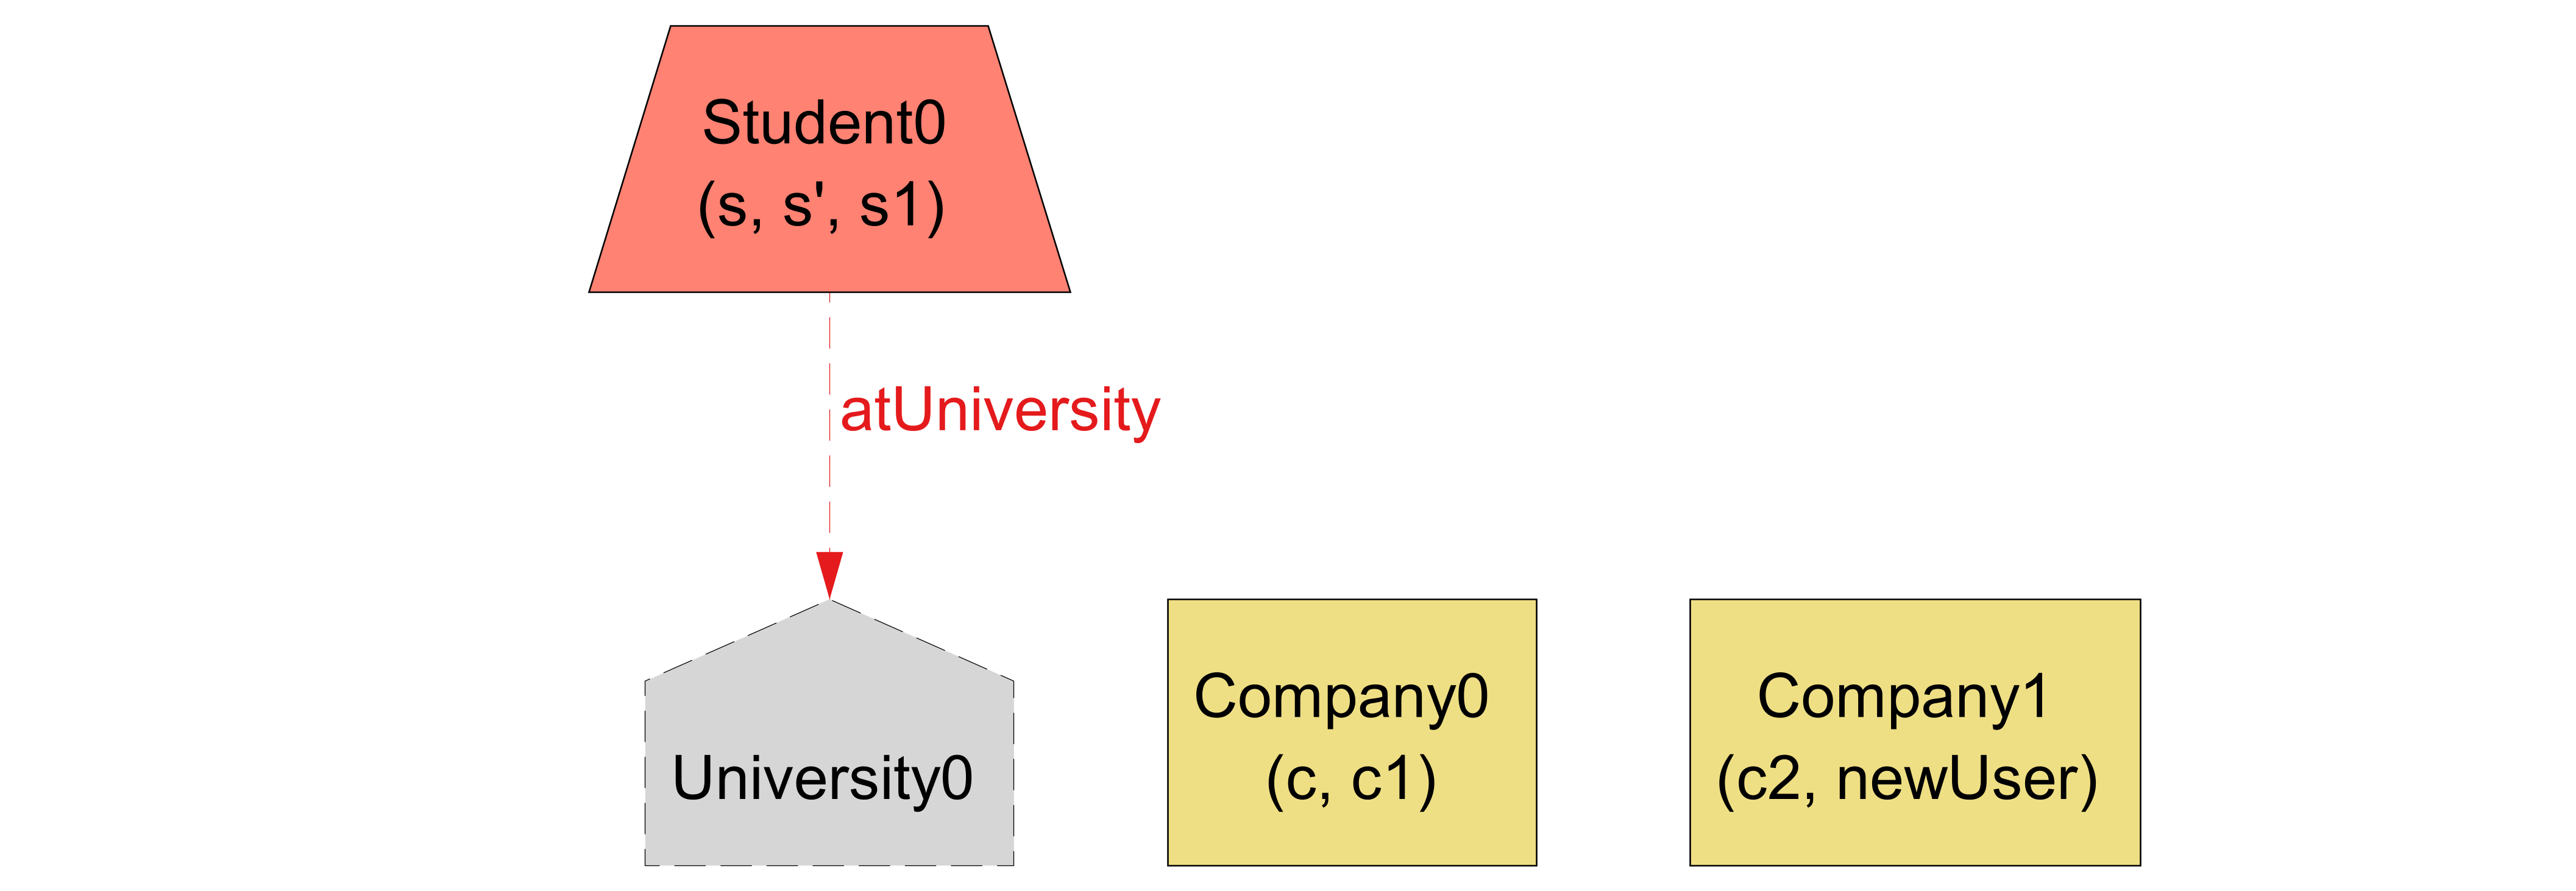
\includegraphics[width=0.5\linewidth]{LaTeXCode/images/Alloy/dynamicWorld_step1.png}
        \caption{Example Dynamic World, Step 1} 
        User instances are added to the world as a result of the signUp[] predicate being true.
        \label{fig: dynamicWorld_step1}%
    \end{center}
\end{figure}

\begin{figure}[H]
    \begin{center}
        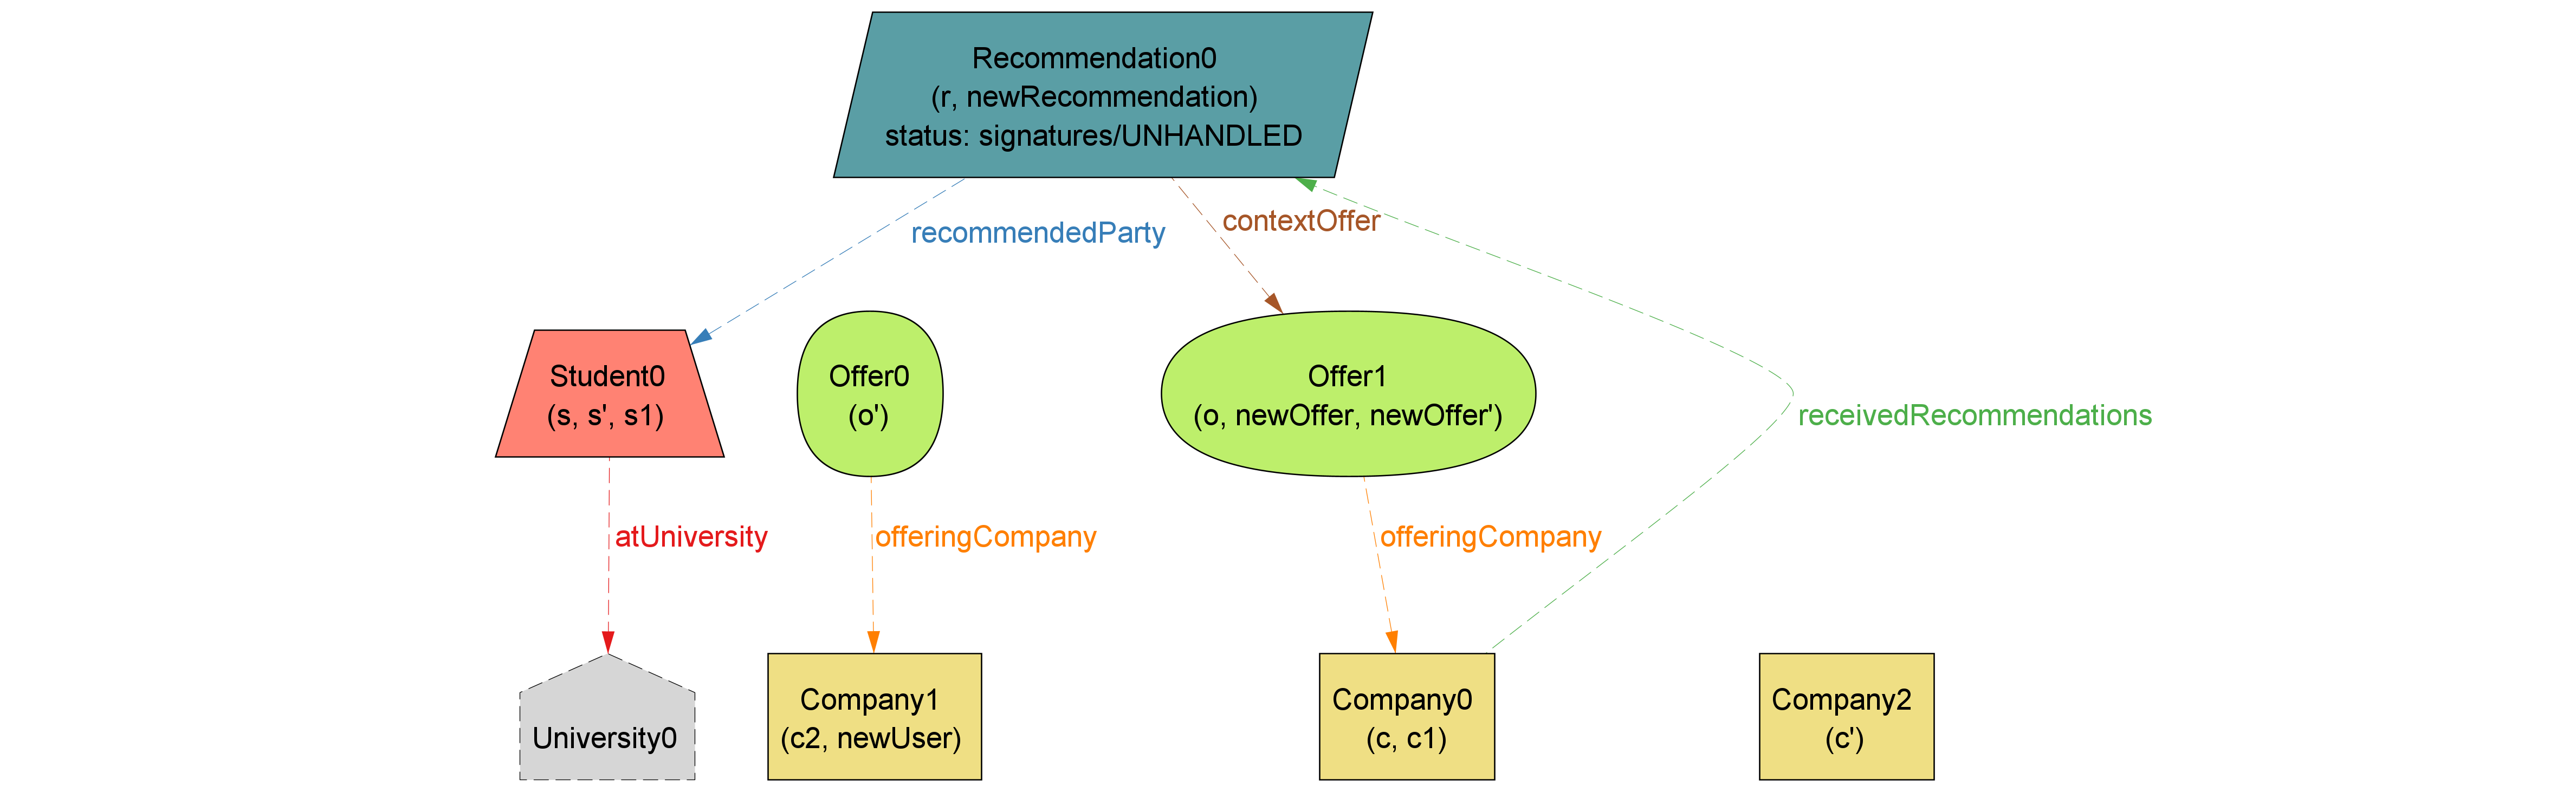
\includegraphics[width=0.7\linewidth]{LaTeXCode/images/Alloy/dynamicWorld_step2.png}
        \caption{Example Dynamic World, Step 2}
        New Offers are added to the world, and a Recommendation is generated as a result.
        \label{fig: dynamicWorld_step2}%
    \end{center}
\end{figure}

\begin{figure}[H]
    \begin{center}
        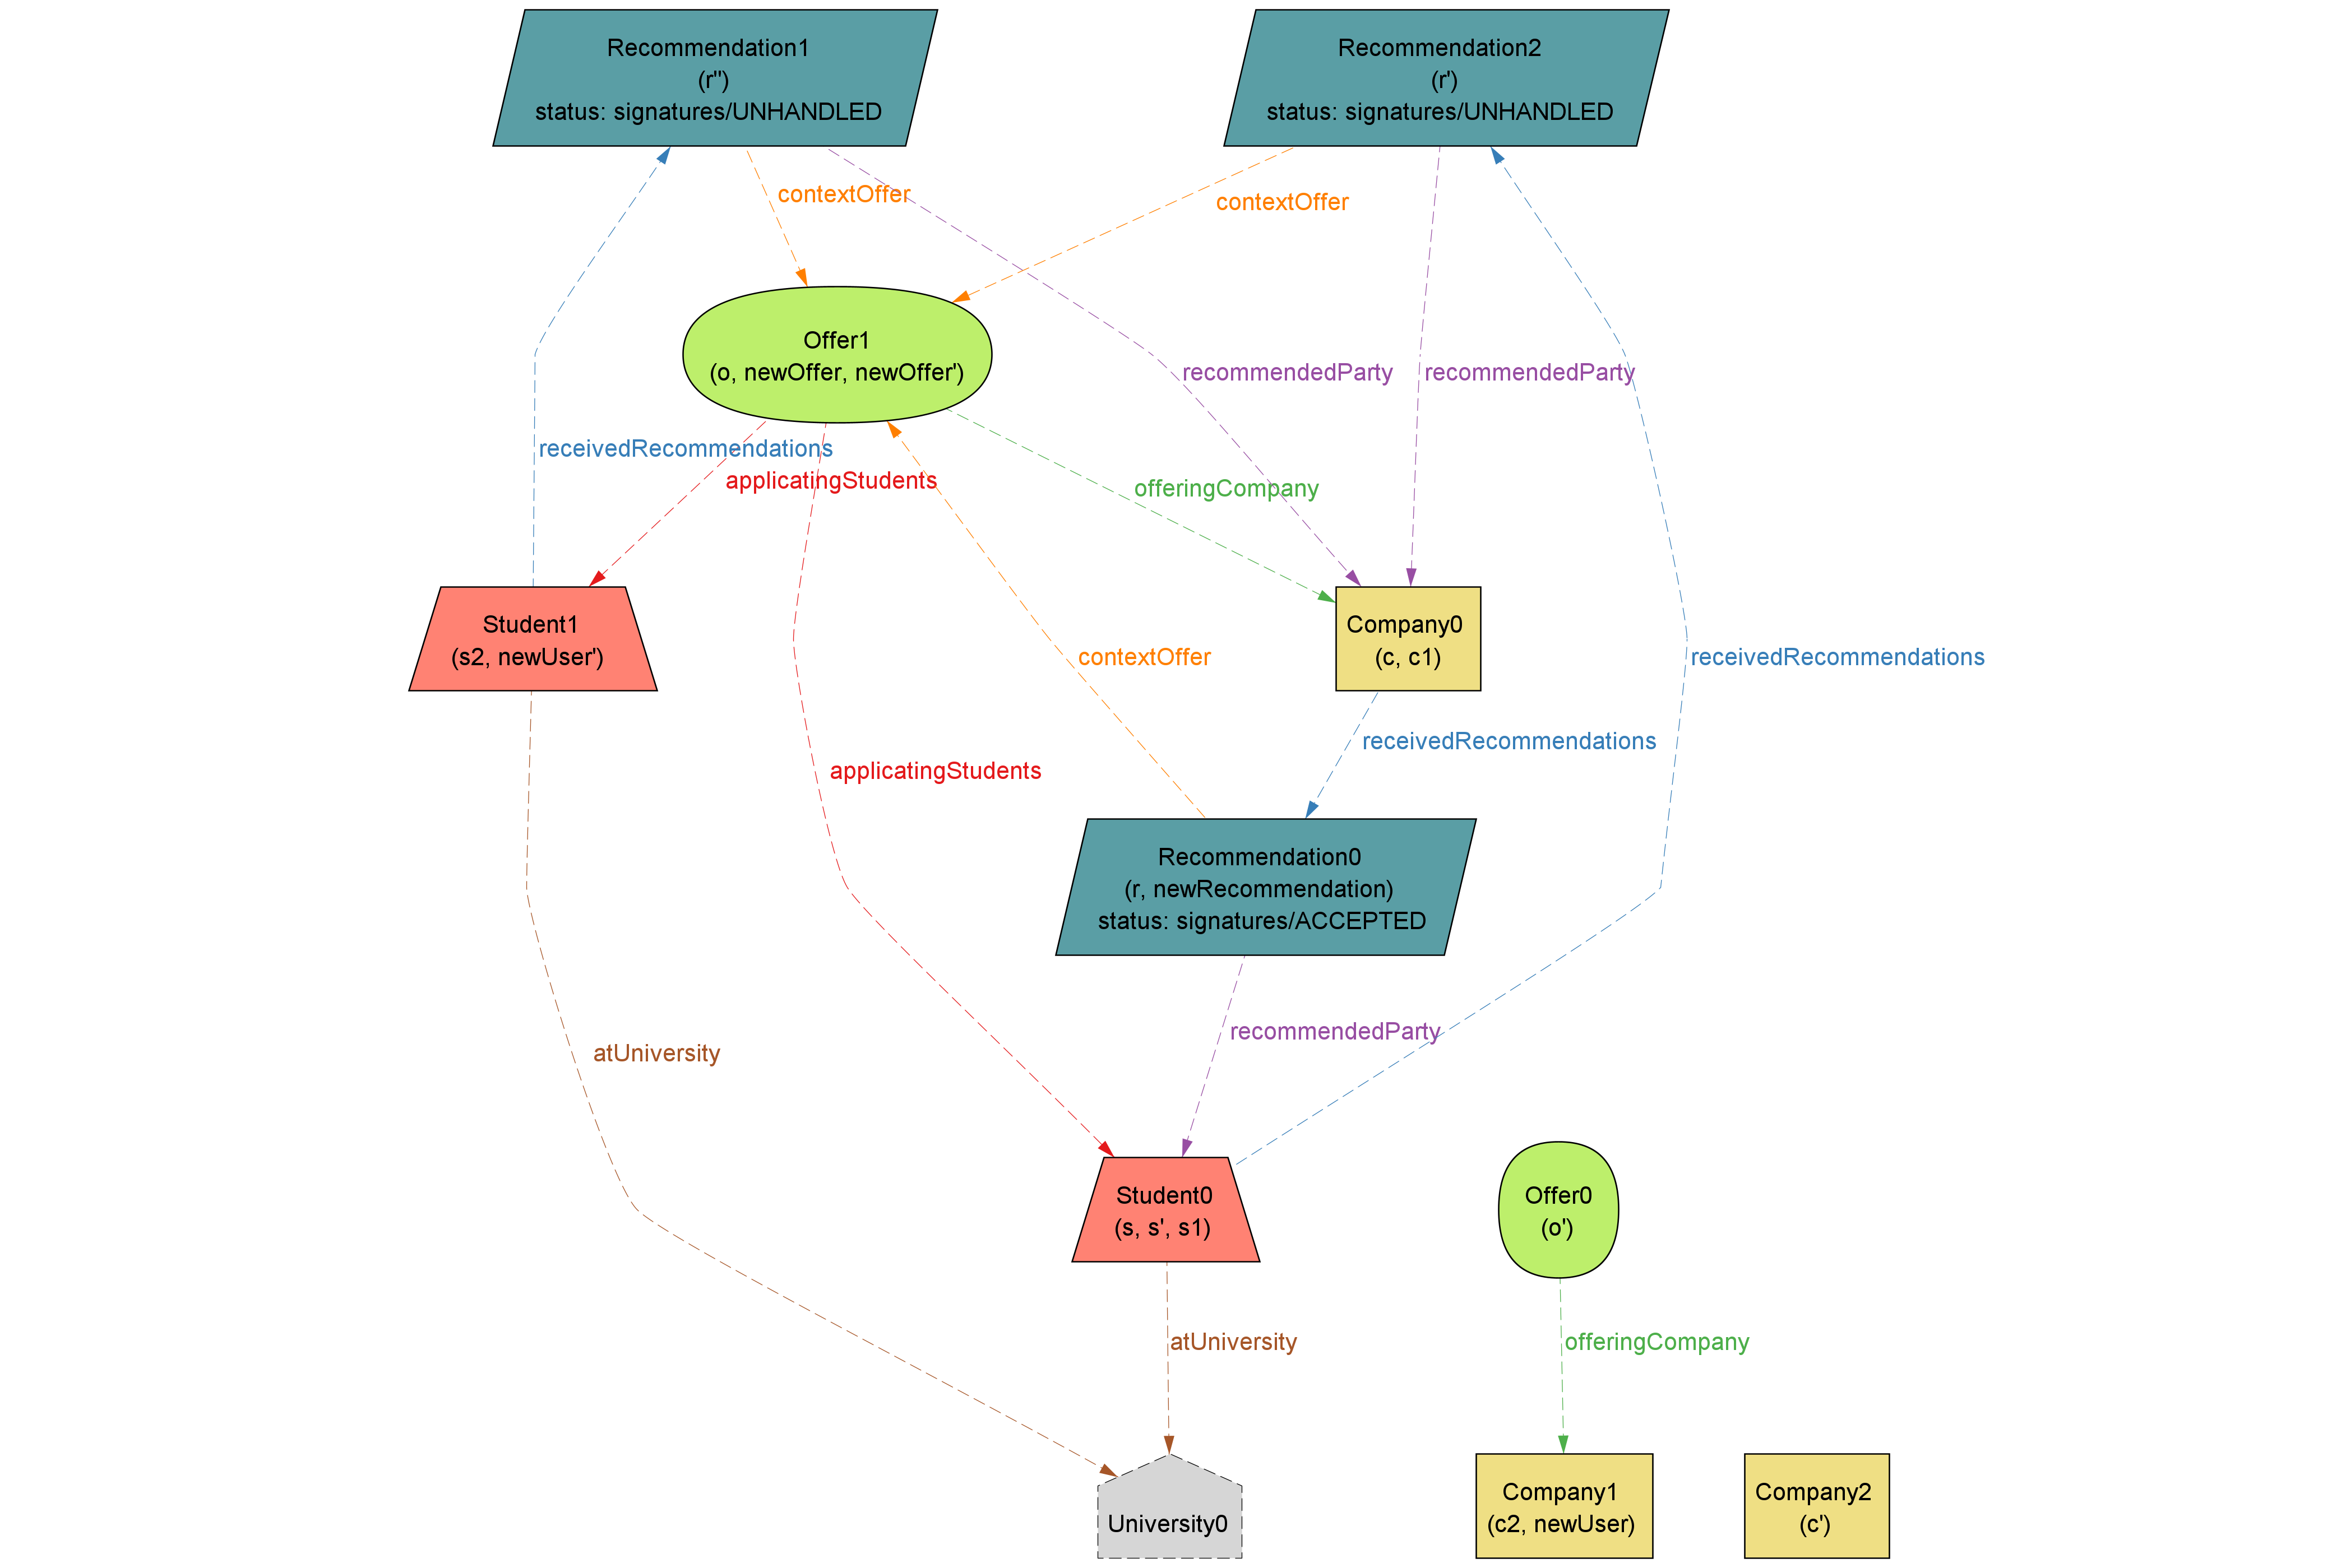
\includegraphics[width=0.7\linewidth]{LaTeXCode/images/Alloy/dynamicWorld_step3_labels.png}
        \caption{Example Dynamic World, Step 3}
        New Users are added to the world; a Company accepts a Recommendation about a Student who doesn't have a reciprocal Recommendation in that context, causing one to be generated.
        \label{fig: dynamicWorld_step3}%
    \end{center}
\end{figure}

\begin{figure}[H]
    \begin{center}
        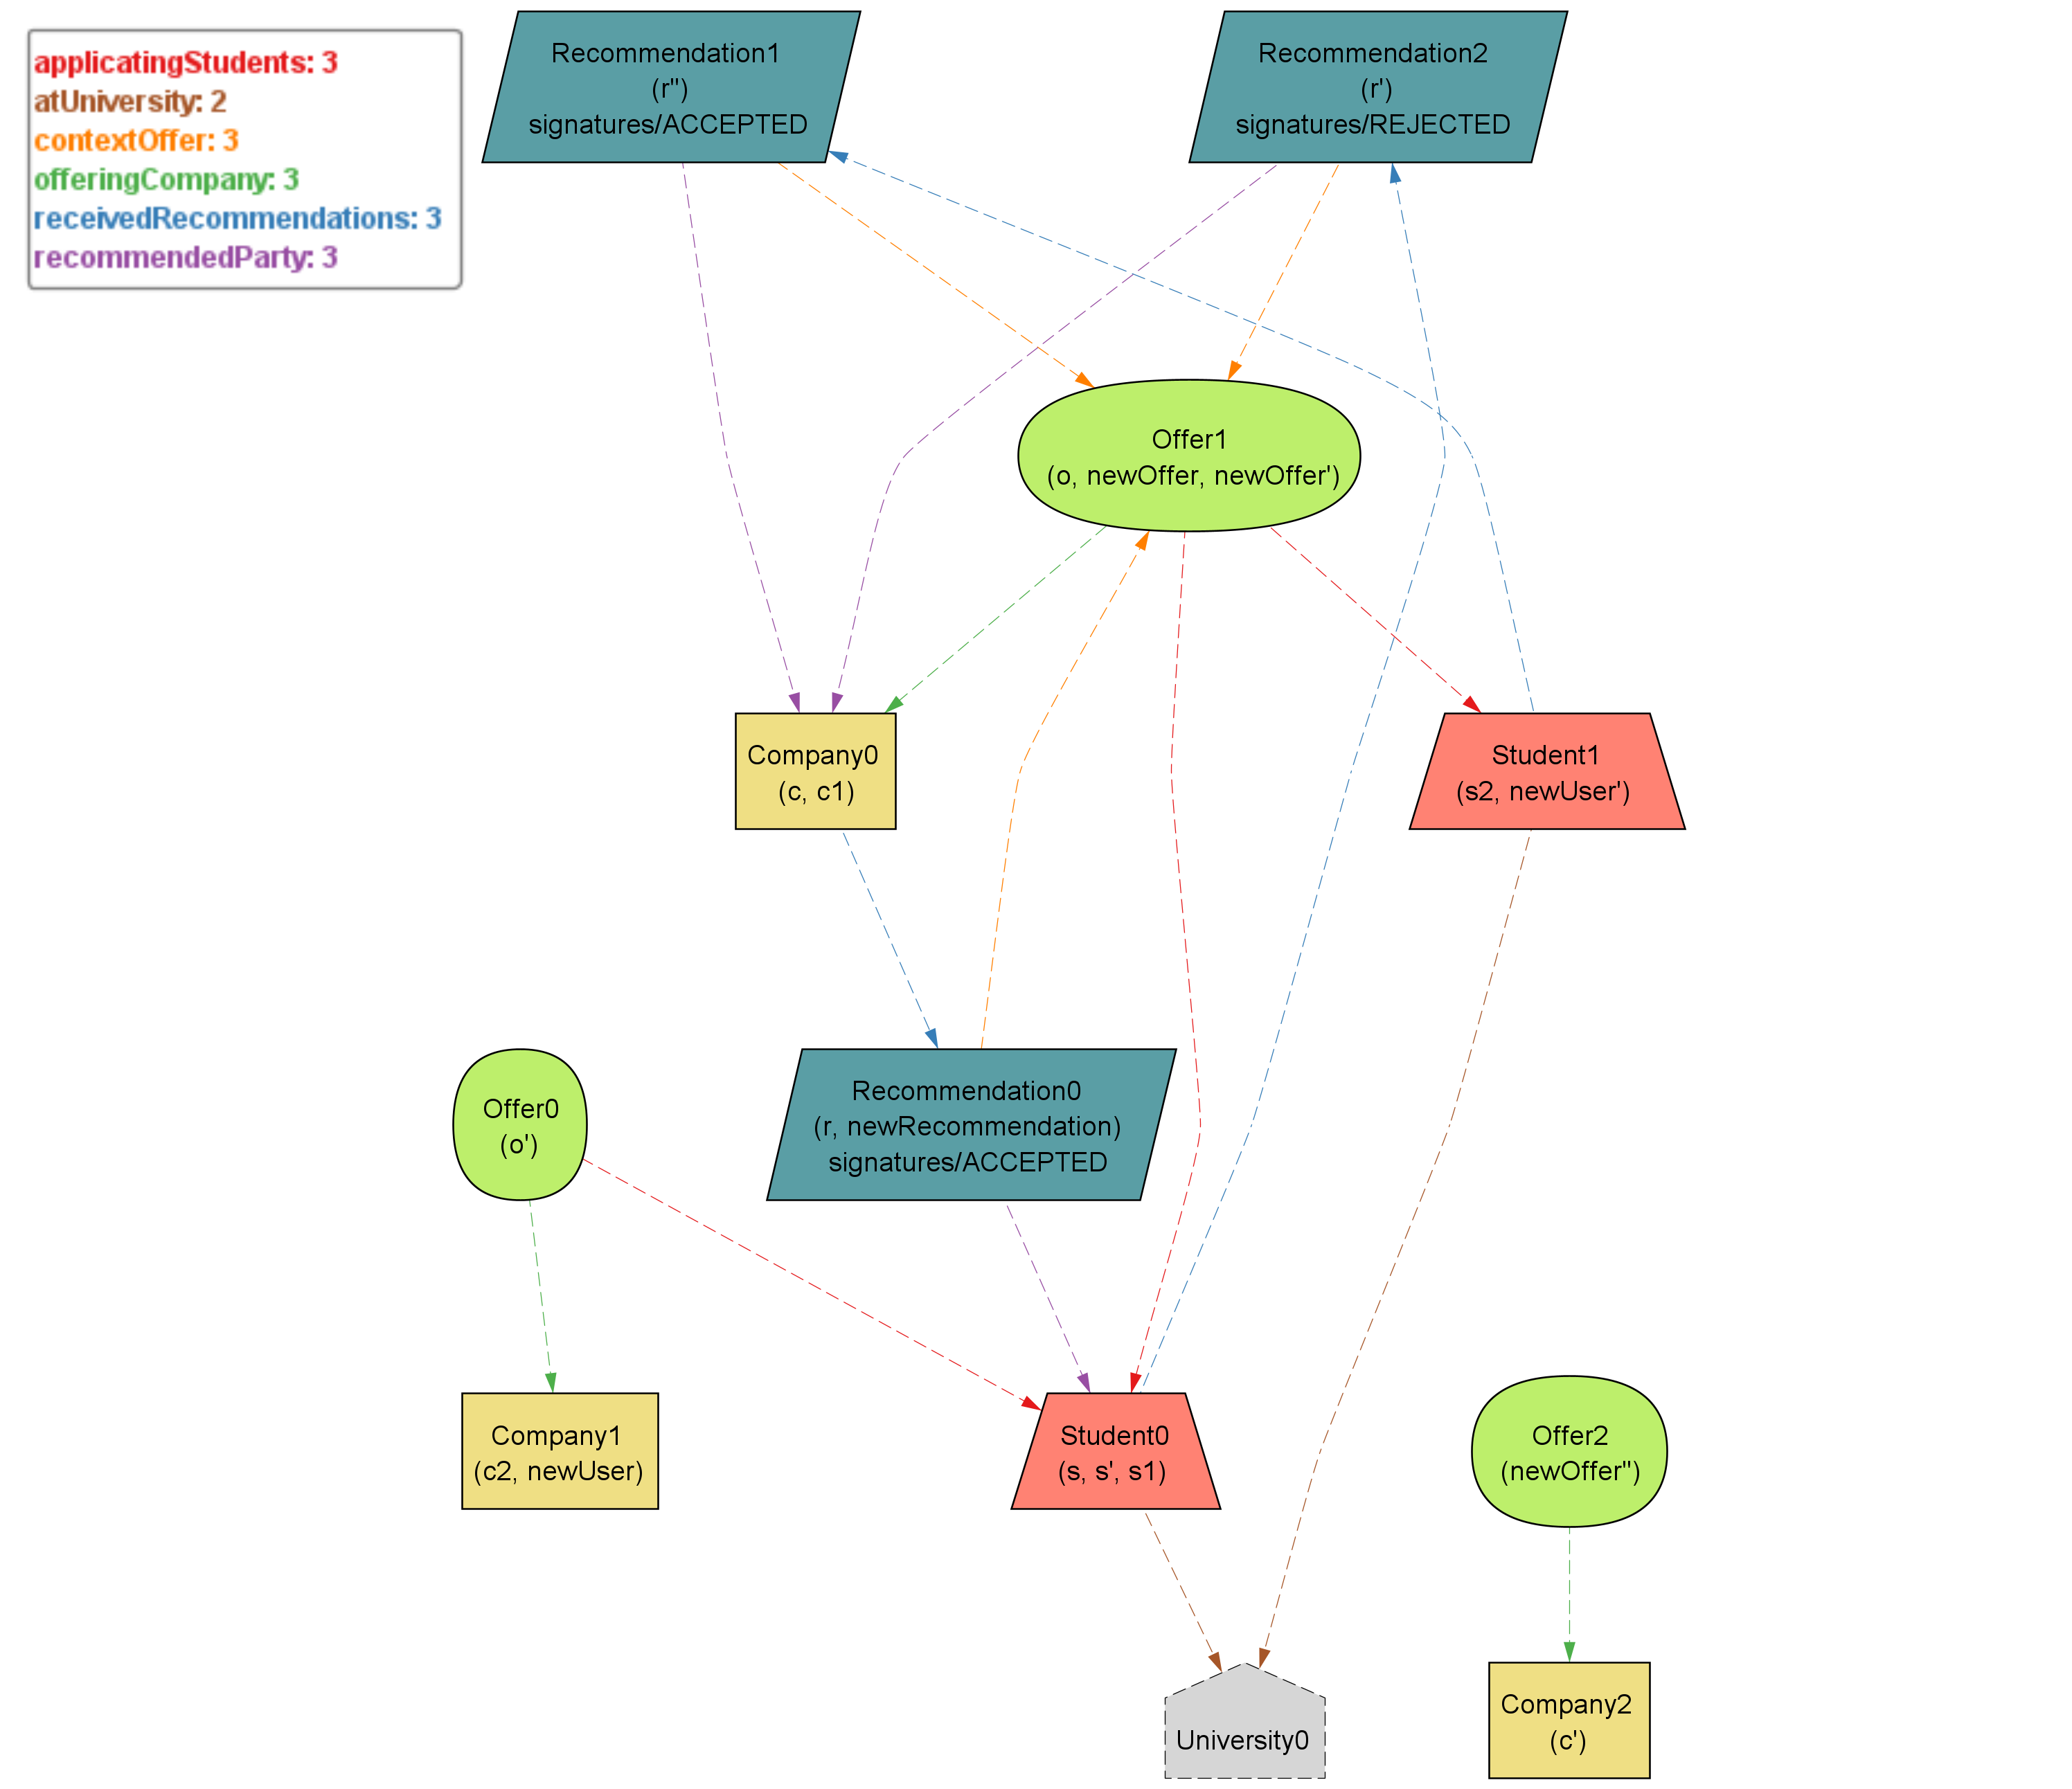
\includegraphics[width=1\linewidth]{LaTeXCode/images/Alloy/dynamicWorld_step4_with_legenda.png}
        \caption{Example Dynamic World, Step 4}
         A Student applies spontaneously to an Offer without passing for a corresponding Recommendation; another Student accepts a Recommendation instead, forcibly applying to the Offer in the context of the Recommendation; a Company rejects a recommendation; a Company without Offers posts a new Offer.
        \label{fig: dynamicWorld_step4}%
    \end{center}
\end{figure}

\begin{comment}
\end{comment}


